\documentclass{article}
\usepackage{graphicx}
\usepackage{fancyhdr}
\usepackage{lipsum}

% Configuración de la página
\pagestyle{fancy}
\fancyhf{}
%\fancyhead[L]{} % Eliminamos la imagen del encabezado en las siguientes páginas
%\fancyhead[R]{Autor: Tu Nombre}
%\fancyhead[C]{Título del Documento}
\fancyfoot[C]{\thepage}

\renewcommand{\headrulewidth}{0pt} % Elimina la línea de la cabecera

\begin{document}

% Primera página
\thispagestyle{fancy} % Aplica el estilo solo a esta página
\begin{titlepage}
    \centering
    \vspace*{2cm}
    {
\includegraphics[width=8cm]{imagenes/logo.png}\par} % Ajusta el nombre de la imagen y su tamaño
    \vspace{1cm}
    {\Huge Título del Documento\par}
    \vspace{2cm}
    {\Large Autor: Tu Nombre\par}
    \vspace{0.5cm}
    {\Large Coautor: Otro Nombre\par} % Agrega el nombre del otro autor
    \vspace{0.5cm}
    {\Large Universidad\par} % Agrega el nombre de la universidad
    \vfill
    {\large \today\par}
\end{titlepage}

\section{Introducción}
Se desea crear un circuito que permita hacer la suma de 16 números guardados en un vector, 
siguiendo el siguiente algoritmo:
\[
\sum_{n=0}^{16} (A_n + A_{n+1})
\]
Entre los componentes que se deben utilizar para desarrollar la solución están los Flip-Flops
tipo \textbf{\textit{JK}}

\section{Almacenamiento}

\subsection{Creación del Vector}
Se creó una unidad de almacenamiento el cual pudiera contener un número de 8 bits y a la vez 
permitirá almacenar un número predeterminado, hasta que llegara el nuevo número por el que se reemplazaría.
\begin{figure}[h] % "h" indica que la figura se coloque aquí, aunque LaTeX puede ajustar su posición
    \centering
    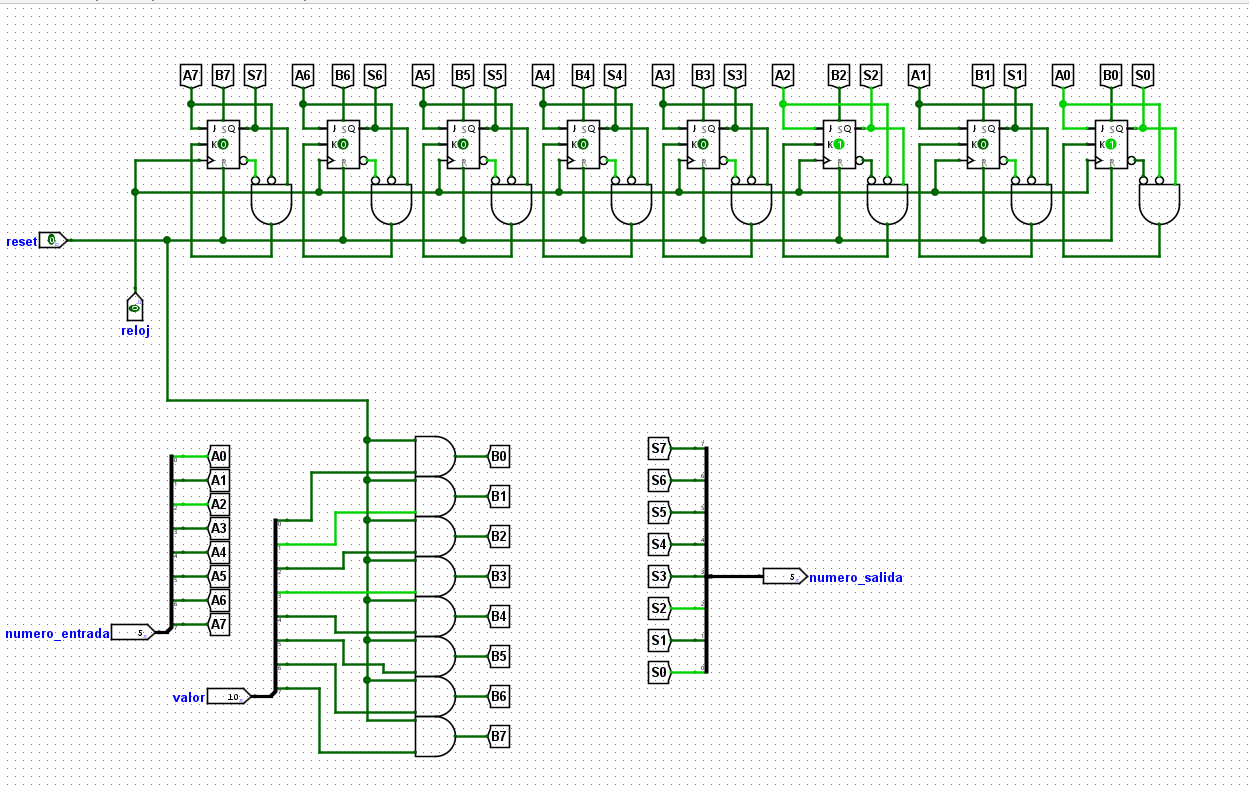
\includegraphics[width=0.8\textwidth]{imagenes/unidad_almacenamiento.png} % Ajusta el nombre de la imagen y el ancho según sea necesario
    \caption{Unidad de almacenamiento} % Agrega la leyenda aquí
    \label{fig:arreglo} % Etiqueta para hacer referencia a la figura en el texto
\end{figure}

Así, de esta manera se podría crear de forma sencilla el vector de 16 posiciones y para el cual se permitiría 
almacenar números predeterminados. Además, se implementó una lógica para que solo escribiera en los arreglos 
correctos según la posición solicitada por el algoritmo y diario se retorne los numeros $A_n$ y $A_{n+1}$

\begin{figure}[h] % "h" indica que la figura se coloque aquí, aunque LaTeX puede ajustar su posición
    \centering
    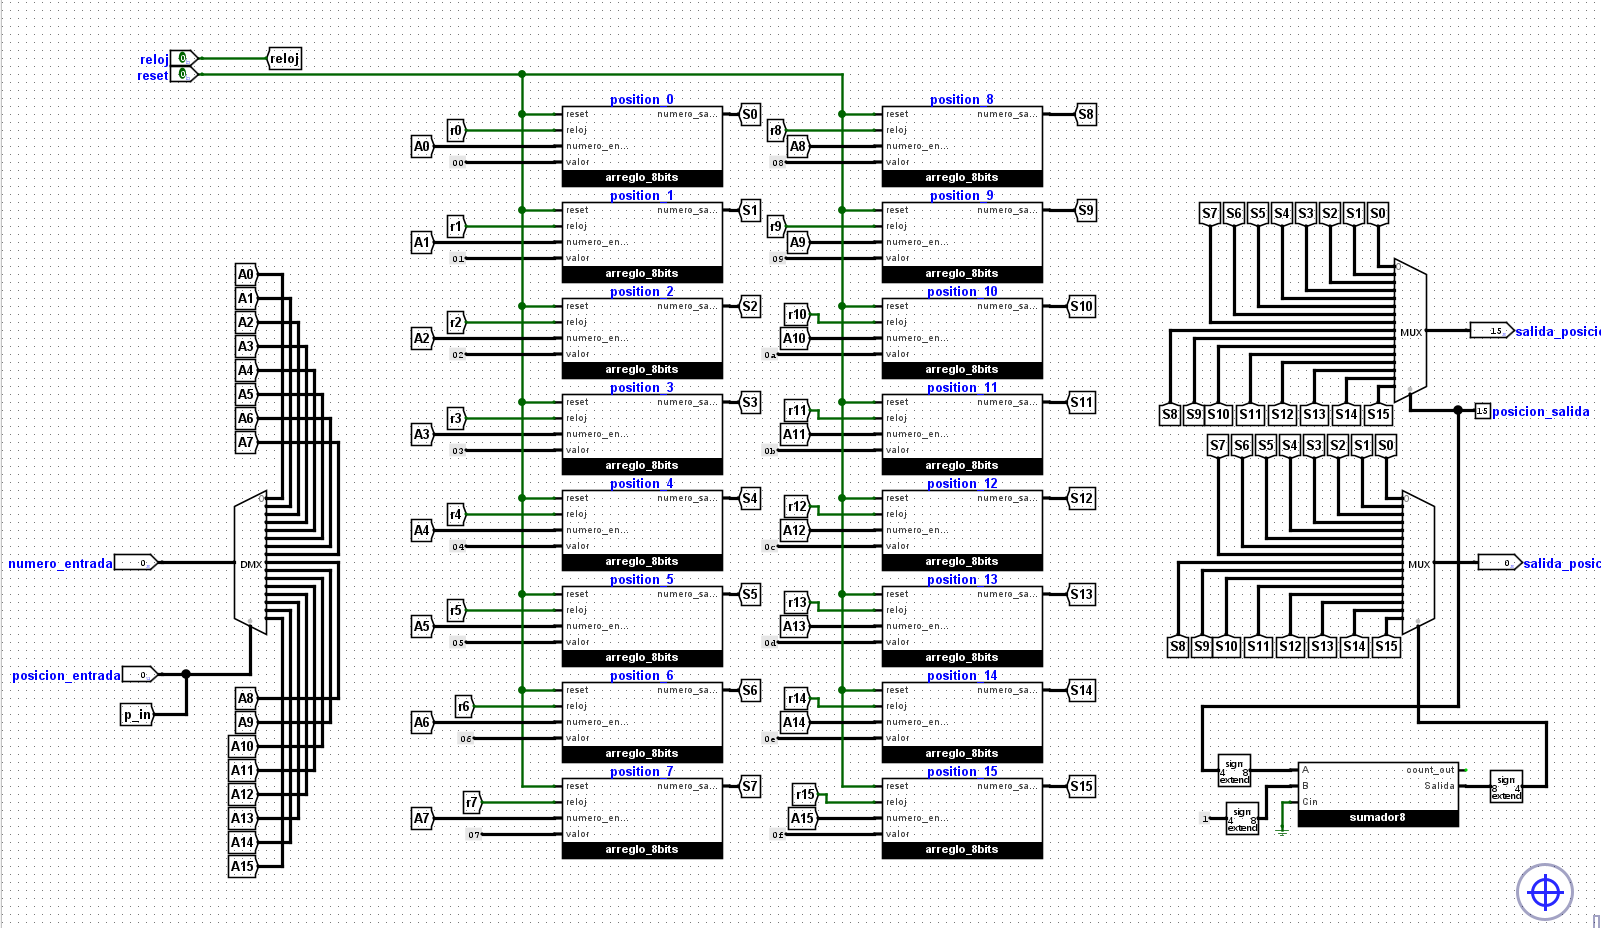
\includegraphics[width=0.8\textwidth]{imagenes/vector.png} % Ajusta el nombre de la imagen y el ancho según sea necesario
    \caption{Vector de 16 posiciones} % Agrega la leyenda aquí
    \label{fig:arreglofull} % Etiqueta para hacer referencia a la figura en el texto
\end{figure}
\newpage
\section{Sumador}
Se construye primero un sumador de un bit full y con base a este se procede a construir uno para 8 bits 
que es la cantidad máxima para este ejercicio.
\begin{figure}[h]
    \centering
    \begin{minipage}{0.45\textwidth} % ajusta el ancho de la primera imagen
      \centering
      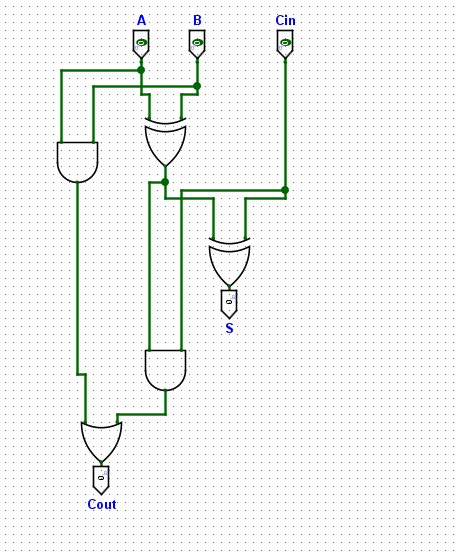
\includegraphics[width=\linewidth]{imagenes/sumador.png} % reemplaza "imagen1" con el nombre de tu primera imagen
      \caption{Sumador completo de 1 bit}
      \label{fig:sumador}
    \end{minipage}
    \hfill
    \begin{minipage}{0.45\textwidth} % ajusta el ancho de la segunda imagen
      \centering
      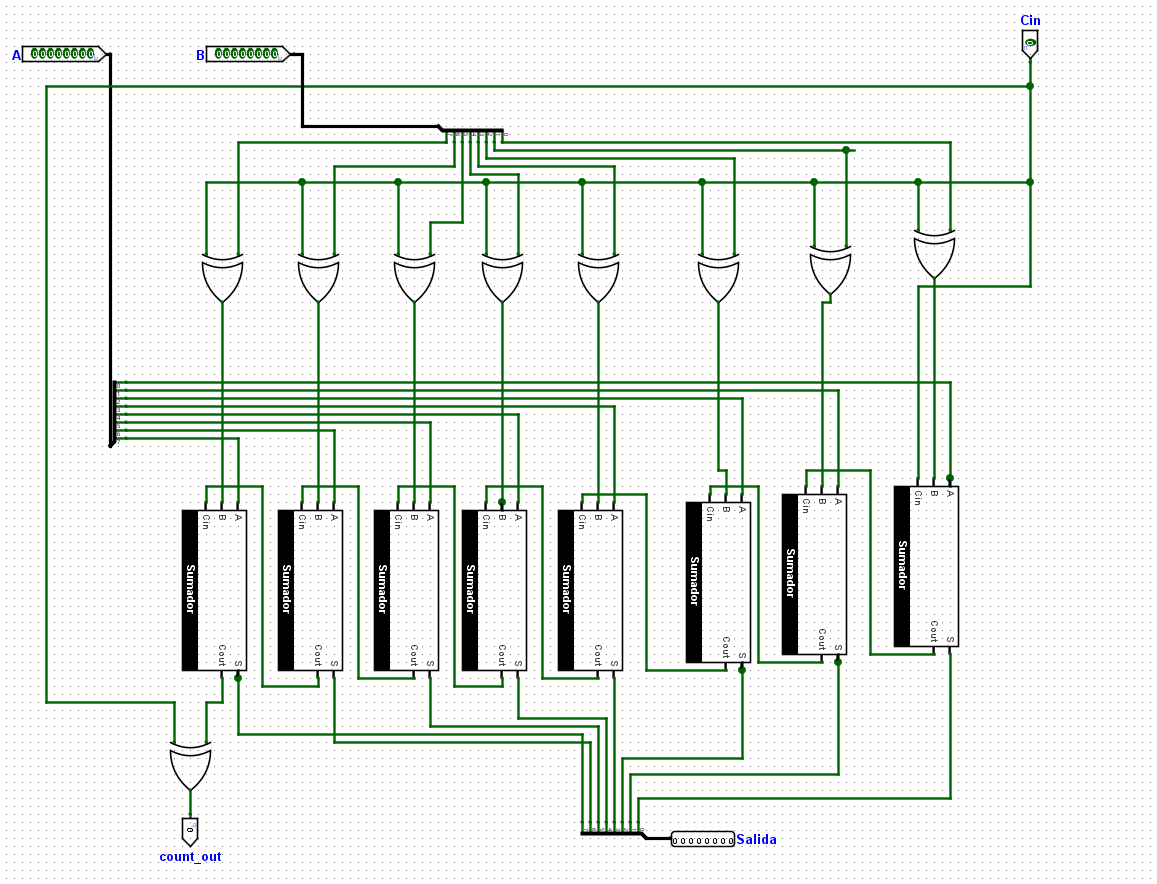
\includegraphics[width=\linewidth]{imagenes/sumador8.png} % reemplaza "imagen2" con el nombre de tu segunda imagen
      \caption{Sumador completo de 8 bits}
      \label{fig:sumador8}
    \end{minipage}
\end{figure}

\section{Contadores}
\subsection{Contador unidad}
Para este ejercicio se creó un contador de 4 bits (16 posiciones posibles) con el flip-flop tipo Jk 
conectados en cascada, el cual ayudaría para saber qué posición del vector guardar los datos, en que 
fase del algoritmo se encuentra y el estado de la máquina.
\begin{figure}[h] % "h" indica que la figura se coloque aquí, aunque LaTeX puede ajustar su posición
    \centering
    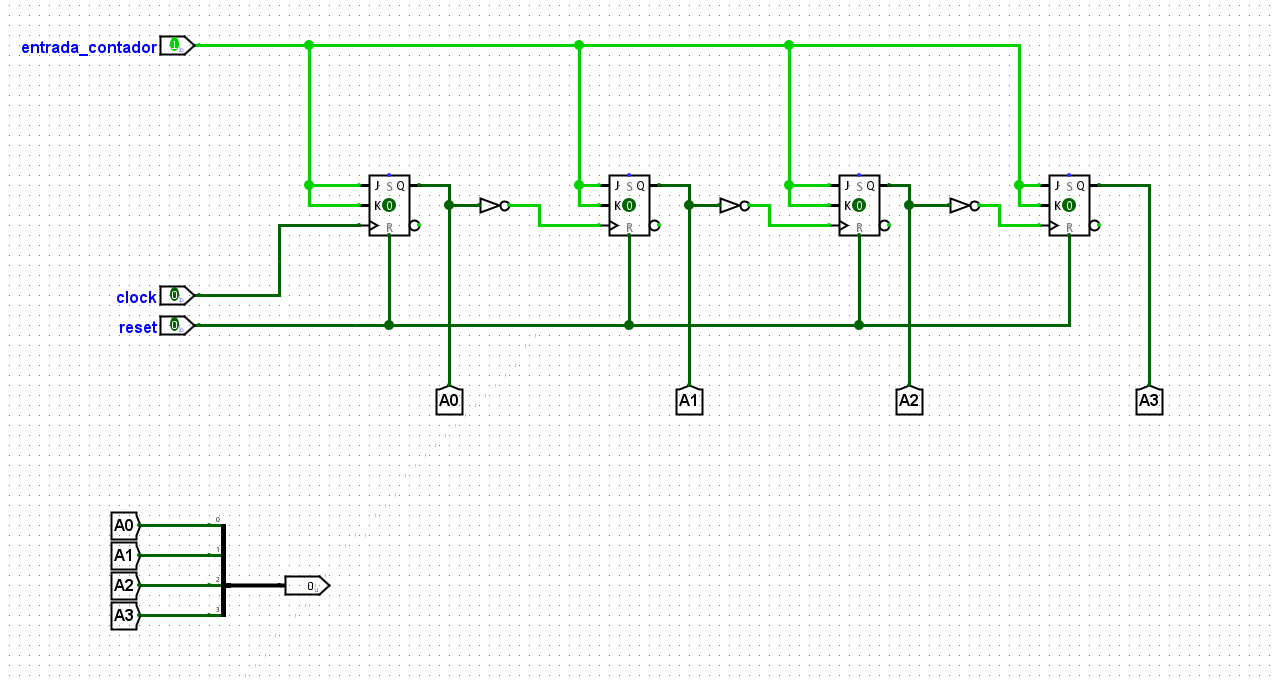
\includegraphics[width=0.8\textwidth]{imagenes/contador.png} % Ajusta el nombre de la imagen y el ancho según sea necesario
    \caption{Contador de 4 bits} % Agrega la leyenda aquí
    \label{fig:contador} % Etiqueta para hacer referencia a la figura en el texto
\end{figure}

\subsection{Contador par}

\end{document}
